\chapter{URG of the single-impurity Anderson model: RG flows and fixed point Hamiltonian}
\label{siamurg}
\section{Brief description of the single-impurity Anderson model}
The model is the usual single-impurity Anderson model Hamiltonian.
\begin{equation}\begin{aligned}
	\label{andham}
	\mathcal{H} = \sum_{k\sigma}\epsilon_k \hat n_{k\sigma} + \sum_{k\sigma} \left(V_{k} c^\dagger_{k\sigma} c_{d\sigma} + h.c.\right) + \epsilon_{d}\sum_\sigma  \hat n_{d\sigma} +  U \hat n_{d\uparrow} \hat n_{d\downarrow}
\end{aligned}\end{equation}
To allow the calculation of both particle and hole kinetic energies, we will write the kinetic energy part as \(\sum_{k\sigma}\epsilon_k \tau_{k\sigma}\), where \(\tau = \hat n - \frac{1}{2}\) and drop the extra constant part.
\begin{equation}
	\label{model:siam}
	\mathcal{H} = \sum_{k\sigma}\epsilon_k \tau_{k\sigma} + \sum_{k\sigma} \left(V_{k} c^\dagger_{k\sigma} c_{d\sigma} + h.c.\right) + \epsilon_{d}\sum_\sigma  \hat n_{d\sigma} +  U \hat n_{d\uparrow} \hat n_{d\downarrow}
\end{equation}
\section{Calculation of renormalisation}
The renormalisation is
\begin{equation}\begin{aligned}
\label{newh}
c^\dagger_{q\beta}T \frac{1}{\omega - H^D}T^\dagger c_{q\beta} + T^\dagger c_{q\beta}\frac{1}{\omega^\prime - H^D}c^\dagger_{q\beta}T
\end{aligned}\end{equation}
We will be decoupling an electron \(q\beta\) at the energy shell \(\epsilon_q = \pm D\). The diagonal part (that comes down in the denominator) is
\begin{equation}\begin{aligned}
	\label{term1}
H^D = \epsilon_q \tau_{q\beta} + \epsilon_{d}\hat n_{d\beta} +  U \hat n_{d\beta} \hat n_{d\bar\beta}
\end{aligned}\end{equation}
The off-diagonal part is
\begin{equation}\begin{aligned}
	c^\dagger_{q\beta}T = V_q c^\dagger_{q\beta}c_{d\beta}
\end{aligned}\end{equation}

The renormalisation from a single electron \(q\beta\) is
\begin{equation}\begin{aligned}
	\Delta H &= c^\dagger_{q\beta}c_{d\beta} \frac{1|V_q|^2}{\omega - H^D}c_{d\beta}^\dagger c_{q\beta} + c_{d\beta}^\dagger c_{q\beta}\frac{1|V_q|^2}{\omega^\prime - H^D}c^\dagger_{q\beta}c_{d\beta} \\
		 &= c^\dagger_{q\beta}c_{d\beta} \frac{|V_q|^2}{\omega - D/2 - \epsilon_d - U \hat n_{d\bar\beta}}c_{d\beta}^\dagger c_{q\beta} + c_{d\beta}^\dagger c_{q\beta}\frac{|V_q|^2}{\omega^\prime - D/2}c^\dagger_{q\beta}c_{d\beta}\\
		 &=  \frac{\hat n_{q\beta}\left( 1 - \hat n_{d\beta} \right) |V_q|^2}{\omega - D/2 - \epsilon_d - U \hat n_{d\bar\beta}} + \frac{\hat n_{d\beta}\left( 1 - \hat n_{q\beta} \right) |V_q|^2}{\omega^\prime - D/2}
\end{aligned}\end{equation}

For comparing the two \(\omega\)s, we will use the relation eq.~\ref{omegarel}: \(\omega_0^1 + \omega^1_0 = H^D_0 + H^D_1\) where \(\omega_0^1 = \omega^\prime\). \(\omega^1_0\) however is not \(\omega\). This is because the relation assumes the \(\omega\)s to be calculated at the same energy - while \(\omega^\prime\) is calculated at energy \(-D\), \(\omega\) is at energy \(D\). The \(\omega_0^1\) should hence be the \(\omega\) at energy \(-D\), which is \(-\omega\). With this in mind, the relation says
\begin{equation}\begin{aligned}
	\omega^\prime - \omega = D/2 + \epsilon_d + U \hat n_{d\beta} - D/2 
\end{aligned}\end{equation}
This gives an expression of \(\omega^\prime\) in terms of \(\omega\). Substituting this into \(\Delta H\)  gives
\begin{equation}\begin{aligned}
	\Delta H &=  \frac{\hat n_{q\beta}\left( 1 - \hat n_{d\beta} \right) |V_q|^2}{\omega - D/2 - \epsilon_d - U \hat n_{d\bar\beta}} + \frac{\hat n_{d\beta}\left( 1 - \hat n_{q\beta}\right)|V_q|^2}{\omega - D/2 +\epsilon_d + U \hat n_{d\bar\beta}}
\end{aligned}\end{equation}
The total renormalisation from the entire shell \(\pm D\) is
\begin{equation}\begin{aligned}
	\label{vanilla:siam:ren}
	\Delta H &=  \sum_{q\beta}|V_q|^2\left[\frac{\hat n_{q\beta}\left( 1 - \hat n_{d\beta} \right) }{\omega - D/2 - \epsilon_d - U \hat n_{d\bar\beta}} + \frac{\hat n_{d\beta}\left( 1 - \hat n_{q\beta}\right)}{\omega - D/2 +\epsilon_d + U \hat n_{d\bar\beta}}\right] \\
		 &= \sum_q |V_q|^2 \left[\frac{\left(1 - \hat n_{d\beta}\right)\hat n_{d\overline\beta}}{\omega - \frac{1}{2}\epsilon_q - \epsilon_d - U} + \frac{\left(1 - \hat n_{d\beta}\right)\left( 1-\hat n_{d\overline\beta} \right)}{\omega - \frac{1}{2}\epsilon_q - \epsilon_d} + \frac{\hat n_{d\beta} \hat n_{d\overline\beta}}{\omega - \frac{1}{2}\epsilon_q + \epsilon_d + U} + \frac{\hat n_{d\beta}\left( 1- \hat n_{d\overline\beta}\right) }{\omega - \frac{1}{2}\epsilon_q + \epsilon_d}\right]
\end{aligned}\end{equation}
\section{Scaling equations for the SIAM}
Once we have the renormalisation for decoupling one electronic or hole state, we can just sum over the spins and momenta to get the total renormalisation upon decoupling the entire shells \(\pm \epsilon_q\). From the structure of \(\Delta \mathcal{H}\) in eq.~\ref{vanilla:siam:ren}, we can see that there are renormalisations to all three configuration energies of the impurity: the doublon energy \(E_2\) corresponding to the state  \(\hat n_{d\beta}\hat n_{d\overline\beta}\), the single energy \(E_1\) corresponding to (\(\hat n_{d\beta}(1 - \hat n_{d\overline\beta}) + \hat n_{d\overline\beta}(1 - \hat n_{d\beta})\), and the holon energy \(E_0\) corresponding to \((1 - \hat n_{d\beta})(1 - \hat n_{d\overline\beta}) + \hat n_{d\overline\beta}(1 - \hat n_{d\beta})\).
\begin{equation}\begin{aligned}
	\label{urg-siam}
	\Delta E_2 &= +2\sum_{q}\frac{|V_q|^2}{\omega - \frac{1}{2}\epsilon_q + \epsilon_d + U }\\
	\Delta E_1 &= +\sum_{q}\frac{|V_q|^2}{\omega - \frac{1}{2}\epsilon_q + \epsilon_d} + \sum_{q}\frac{|V_q|^2}{\omega - \frac{1}{2}\epsilon_q - \epsilon_d - U}\\
	\Delta E_0 &= +2\sum_{q}\frac{|V_q|^2}{\omega - \frac{1}{2}\epsilon_q - \epsilon_d}
\end{aligned}\end{equation}
Using the relations \(\epsilon_d = E_1 - E_0\) and \(U = E_2 + E_0 - 2E_1\), we can write
\begin{equation}\begin{aligned}
	\Delta \epsilon_d &= +\sum_{q}\frac{|V_q|^2}{\omega - \frac{1}{2}\epsilon_q + \epsilon_d} + \sum_{q}\frac{|V_q|^2}{\omega - \frac{1}{2}\epsilon_q - \epsilon_d - U} - 2\sum_{q}\frac{|V_q|^2}{\omega - \frac{1}{2}\epsilon_q - \epsilon_d}\\
	\Delta U &= \sum_{q}\frac{2|V_q|^2}{\omega - \frac{1}{2}\epsilon_q + \epsilon_d + U } + \sum_{q}\frac{2|V_q|^2}{\omega - \frac{1}{2}\epsilon_q - \epsilon_d} - \sum_{q}\frac{2|V_q|^2}{\omega - \frac{1}{2}\epsilon_q + \epsilon_d} - \sum_{q}\frac{2|V_q|^2}{\omega - \frac{1}{2}\epsilon_q - \epsilon_d - U}\\
\end{aligned}\end{equation}
\section{Connection to poor man's scaling}\label{urg2pms}
To obtain the results of Poor Man's scaling \cite{haldane1978scaling}\cite{jefferson_1977},  we can look at various regimes. First we look at the case when both \(\epsilon_d\) and \(U\) are small such that both the singly-occupied and doubly-occupied subspaces of the impurity are comfortably inside the bandwidth, \(U,\epsilon_d \ll \epsilon_q\). We can then ignore the \(\epsilon_d\) and \(U\) in the denominator compared to the \(\epsilon_q\).
\begin{equation}\begin{aligned}
\Delta \epsilon_d &= \sum_{q}\frac{|V_q|^2}{\omega - \frac{1}{2}\epsilon_q} + \sum_{q}\frac{|V_q|^2}{\omega - \frac{1}{2}\epsilon_q} - 2\sum_{q}\frac{|V_q|^2}{\omega - \frac{1}{2}\epsilon_q}\\
\Delta U &= 2\sum_{q}\frac{|V_q|^2}{\omega - \frac{1}{2}\epsilon_q} + 2\sum_{q}\frac{|V_q|^2}{\omega - \frac{1}{2}\epsilon_q} - 2\sum_{q}\frac{|V_q|^2}{\omega - \frac{1}{2}\epsilon_q} - 2\sum_{q}\frac{|V_q|^2}{\omega - \frac{1}{2}\epsilon_q}
\end{aligned}\end{equation}
Assuming the upper and lower band edges are symmetrical such that \(\sum_{-D} = \sum_D\), we get \(\Delta \epsilon_d = \Delta U = 0\). 

In the regime \(U \gg \epsilon_q \gg \epsilon_d\), the doubly-occupied state is far above the bandwidth. We can now ignore the terms that have \(U\) in the denominator. We get
\begin{equation}\begin{aligned}
\Delta \epsilon_d &= \sum_{q}\frac{|V_q|^2}{\omega - \frac{1}{2}\epsilon_q} - 2\sum_{q}\frac{|V_q|^2}{\omega - \frac{1}{2}\epsilon_q}\\
\Delta U &= 2\sum_{q}\frac{|V_q|^2}{\omega - \frac{1}{2}\epsilon_q}  - 2\sum_{q}\frac{|V_q|^2}{\omega - \frac{1}{2}\epsilon_q} 
\end{aligned}\end{equation}
Again assuming symmetrical upper and lower edges, and isotropic dispersion \(\epsilon_q=D\) and \(\sum_q |V|^2 = \frac{\Delta}{\pi}|\delta D|\), we get
\begin{equation}\begin{aligned}
\Delta U &= 0\\
\delta \epsilon_d &= -\frac{\Delta}{\pi}\frac{1}{\omega - \frac{1}{2} D}
\end{aligned}\end{equation}
There we replaced the difference symbol \(\Delta\) with \(\delta\) to avoid confusion with the hybridisation \(\Delta \sim \sum V^2\). For low quantum fluctuations, we can ignore the renormalisation in the couplings and replace \(\omega\) with the initial conduction electron energy: \(\omega = \epsilon_q\tau_{q\beta} = -\frac{1}{2} D\).
\begin{equation}\begin{aligned}
\delta \epsilon_d &= \frac{\Delta}{\pi}\frac{\delta D}{D}
\end{aligned}\end{equation}
This is the one-loop scaling equation.
\section{Preservation of particle-hole symmetry}
The Anderson model Hamiltonian, eq.~\ref{andham}, has an impurity particle-hole symmetry for a certain condition of the couplings. To see this, we apply the particle-hole transformation \(c_k \to c^\dagger_k, c_d \to -c^\dagger_d\) to the Hamiltonian. Since we are looking at the impurity symmetry, we will only look at the terms involving the impurity. The particle-hole symmetry of the conduction bath is a separate thing and that requires a specific lattice. Hence we will not consider kinetic energy term in this discussion. The rest of the terms transform as
\begin{gather}
    \epsilon_d \sum_\sigma \hat n_{d\sigma} \to 2\epsilon_d - \epsilon_d \sum_\sigma \hat n_{d\sigma}\label{imp1}\\
U \hat n_{d\uparrow}\hat n_{d\downarrow} \to U \hat n_{d\uparrow}\hat n_{d\downarrow} - U\sum_\sigma \hat n_{d\sigma} + U\label{imp2}\\
\sum_{k\sigma}V(k)c^\dagger_{k\sigma}c_{d\sigma} + hc \to \sum_{k\sigma}-V(k)c_{k\sigma}c^\dagger_{d\sigma} + hc = \sum_{k\sigma}V^*(k)c^\dagger_{k\sigma}c_{d\sigma} + hc \label{hop}
\end{gather}
The impurity-bath hopping term can be made symmetric by making \(V(k)\) real; we would then have, from eq.~\ref{hop},
\begin{equation}\begin{aligned}
	V(k)\left(c^\dagger_{k\sigma}c_{d\sigma} + c^\dagger_{d\sigma}c_{k\sigma}\right)\to V(k)\left(c^\dagger_{d\sigma}c_{k\sigma} + c^\dagger_{k\sigma}c_{d\sigma}\right)
\end{aligned}\end{equation}
The impurity diagonal terms, \(\epsilon_d\) and \(U\), require a specific condition. Combining eqs.~\ref{imp1} and \ref{imp2},
\begin{equation}\begin{aligned}
	\epsilon_d\hat n_{d\sigma} + U\hat n_{d\uparrow}\hat n_{d\downarrow} \to \left(-\epsilon_d - U\right)\hat n_{d\sigma} + U\hat n_{d\uparrow}\hat n_{d\downarrow}
\end{aligned}\end{equation}
We dropped some constant terms in the transformed Hamiltonian. For particle-hole symmetry, the left and right hand sides must be same. The required condition is thus 
\begin{equation}\begin{aligned}
	\label{phs}
\epsilon_d = -\epsilon_d - U \implies \epsilon_d + \frac{1}{2} U = 0
\end{aligned}\end{equation}
\begin{minipage}{0.5\textwidth}
    This same condition can be obtained in a more physical way. If we consider the singly-occupied state of the impurity as the reference state, the doubly-occupied state is the particle-excitation and the vacant state is the hole excitation. The energy of this particle state is \(E_2 = 2\epsilon_d + U\) and that of the hole state is \(E_0 = 0\). Particle-hole symmetry then requires the particle and hole levels to be degenerate, which means \(E_2 = E_0\), and we recover the condition eq.~\ref{phs}.
\end{minipage}
\hfill
\begin{minipage}{0.4\textwidth}
    \centering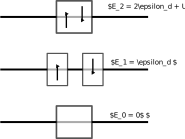
\includegraphics[width=0.8\textwidth]{phsymm.pdf}
    \captionof{figure}{Particle and hole excitations of the impurity}
\end{minipage}

Since the URG is unitary, if we start from a model that is particle-hole symmetric, the RG equations should uphold that symmetry. What this means is that if we have \(\epsilon_d + \frac{1}{2} U = 0\) in the bare model, the new couplings should also satisfy \(\epsilon_d^\prime + \frac{1}{2} U^\prime = 0\). This means we must have 
\begin{equation}\begin{aligned}
	\Delta\left(\epsilon_d + \frac{1}{2} U\right) = 0
\end{aligned}\end{equation}
The quantity \(\gamma = \epsilon_d + \frac{1}{2} U\) is thus an RG-invariant for the particle-hole symmetric model; it does not change under the RG flow. It is often referred to as the asymmetry parameter; it quantifies the asymmetry in the model. We need to check if our equations satisfy this. Looking at the RG equations for \(\epsilon_d\) and \(U\), we can find the RG equation for the asymmetry parameter. The slightly easier way is to just note that the renormalisation in \(E_2\) should be equal to the renormalisation in \(E_0\), in order for p-h symmetry to hold.
\begin{equation}\begin{aligned}
\Delta E_2 &= 2 \frac{\Delta}{\pi}\frac{1}{\omega - D + \epsilon_d + U}, \Delta E_0 &= 2 \frac{\Delta}{\pi}\frac{1}{\omega - D - \epsilon_d}
\end{aligned}\end{equation}
If we start with a particle-hole symmetric model, we will have \(-\epsilon_d = \epsilon_d + U\). Substituting that gives \(\Delta E_2= \Delta E_0\). This shows that the doublon and holon states remain equidistant from the single-particle level, thus maintaining particle-hole symmetry along the flow.
\section{Numerical analysis of the particle-hole symmetric RG equations}
We will specialize to the particle-hole symmetric case, \(2\epsilon_d + U = 0\), and a symmetric energy shell \(\epsilon_q = D\), and look at the scaling behavior of \(\epsilon_d\).
\begin{equation}\begin{aligned}
	\Delta \epsilon_d = -4|V|^2 \frac{\epsilon_d}{\left( \omega - \frac{1}{2}D \right)^2 - \epsilon_d^2}
\end{aligned}\end{equation}
Since the equation is symmetric under \(\epsilon_d \to -\epsilon_d\), we might as well work with the magnitude of the onsite energy:
\begin{equation}\begin{aligned}
	\Delta |\epsilon_d| = -4|V|^2 \frac{|\epsilon_d|}{\left( \omega - \frac{1}{2}D \right)^2 - \epsilon_d^2}
\end{aligned}\end{equation}
Depending on the signature of the denominator, the flows will be either relevant or irrelevant.
\begin{figure}[!htpb]
	\centering
	\includegraphics[width=0.99\textwidth]{../figures/ed_pure_siam.pdf}
	\caption{Left: Irrelevant flow towards \(|\epsilon_d|=0\), at low \(\omega\). Right: Relevant flow towards large \(|\epsilon_d|\), at large \(\omega\). The former can be thought of as the projection of the strong-coupling flow on to the \(\epsilon_d-D\) plane. The latter is the flow towards the local moment fixed point, if we start from a negative \(\epsilon_d\).}
\end{figure}
For the flow to the local moment fixed point, the fixed point value of \(|\epsilon_d|\) grows as we increase the bandwidth. This implies that for a thermodynamically large system, the local moment fixed point will be at \(-\epsilon_d \to \infty\). This behavior is shown in fig.~\ref{edvsD}.
\begin{figure}[htpb]
	\centering
	\includegraphics[width=0.6\textwidth]{../figures/ed_vs_size.pdf}
	\caption{Change in fixed point value of \(|\epsilon_d|\) with system size.}
	\label{edvsD}
\end{figure}
